% ****** Start of file apssamp.tex ******
%
%   This file is part of the APS files in the REVTeX 4.2 distribution.
%   Version 4.2a of REVTeX, December 2014
%
%   Copyright (c) 2014 The American Physical Society.
%
%   See the REVTeX 4 README file for restrictions and more information.
%
% TeX'ing this file requires that you have AMS-LaTeX 2.0 installed
% as well as the rest of the prerequisites for REVTeX 4.2
%
% See the REVTeX 4 README file
% It also requires running BibTeX. The commands are as follows:
%
%  1)  latex apssamp.tex
%  2)  bibtex apssamp
%  3)  latex apssamp.tex
%  4)  latex apssamp.tex
%
\documentclass[twocolumn,superscriptaddress,unsortedaddress,
%runinaddress,
%frontmatterverbose, 
%preprint,
%preprintnumbers,
%nofootinbib,
%nobibnotes,
%bibnotes,
 amsmath,amssymb,
 aps,
%pra,
%prb,
%rmp,
%prstab,
%prstper,
%floatfix,
]{revtex4-2}

\usepackage{graphicx}% Include figure files
\usepackage{dcolumn}% Align table columns on decimal point
\usepackage{bm}% bold math
\usepackage{physics}
\usepackage{xcolor}
% \usepackage{braket}

%\newcommand\abs[1]{\left|#1\right|}
%\newcommand\bra[1]{\left| #1 \right \rangle}
%\newcommand\ket[1]{\left \langle #1 \right |}

\begin{document}

\preprint{APS/123-QED}

\title{Coulomb interaction driven entanglement of electrons on helium}

\author{Niyaz Beysengulov}
\email{beysengu@msu.edu}
\affiliation{Department of Physics and Astronomy, Michigan State University, East Lansing, MI 48824, USA}
\author{Håkon Emil Kristiansen}
\affiliation{Department of Chemistry and Hylleraas Center for Quantum Molecular Sciences, University of Oslo, N-0316 Oslo, Norway}
\author{Øyvind Sigmundson Schøyen}
\affiliation{Department of Physics and Center for Computing in Science Education, University of Oslo, N-0316 Oslo, Norway}
\author{Zachary Stewart}
\affiliation{Department of Chemistry, Michigan State University, East Lansing, MI 48824, USA}
\author{Jared Weidman}
\affiliation{Department of Chemistry, Michigan State University, East Lansing, MI 48824, USA}
\author{Morten Hjorth-Jensen}
\affiliation{Facility for Rare Ion Beams and Department of Physics and Astronomy, Michigan State University, East Lansing, MI 48824, USA}
\affiliation{Department of Physics and Center for Computing in Science Education, University of Oslo, N-0316 Oslo, Norway}
\author{Johannes Pollanen}
\affiliation{Department of Physics and Astronomy, Michigan State University, East Lansing, MI 48824, USA}
\author{Angela Wilson}
\affiliation{Department of Chemistry, Michigan State University, East Lansing, MI 48824, USA}
\begin{abstract}
  Here we describe a method for generating motional entanglement between two electrons trapped above the surface of superfluid helium. In this proposed scheme the electrons are laterally confined via electrostatic gates to create an anharmonic trapping potential 
\end{abstract}

\pacs{02.70.Ss, 31.15.A-, 31.15.bw, 71.15.-m, 73.21.La}


\date{\today}% It is always \today, today,
             %  but any date may be explicitly specified


                              %display desired
\maketitle

%\tableofcontents
\section{Introduction} % Morten + Johannes + Niyaz
Entanglement is the fundamental characteristic that distinguishes
quantum systems composed of two or more coupled objects from their classical counterparts. The study of entanglement in precisely engineered quantum systems with countably many degrees of freedom is at the forefront of modern physics and is a key resource in quantum information science (QIS). This is particularly true in the development of two-qubit logic for quantum computation. In fact, the generation of two-qubit entanglement has been demonstrated in a wide variety of physical systems used in present-day quantum computing, including superconducting circuits~\cite{Steffen1423}, tapped ions~\cite{}, semiconductor quantum dots~\cite{Li809}, color-center defects in diamond~\cite{}, and neutral atoms in optical lattices~\cite{Saffman1010} just to name a few.

\textcolor{blue}{JP will work on this paragraph}Technological advances in QIS, particularly in superconducting qubit and trapped ion experiments, have also created the opportunity to explore the generation of entanglement in emerging QIS systems based on trapped electrons~{}. Some statement of why one would like this kind of thing. Faster electron chain phonons, no screening, so very strong Coloumb interactions. paradigm for studying the role of entanglement produced purely by the Coloumb interaction and what kinds of entanglement protocols are possible.

The system of electrons on helium is quantum non-degenerate, the system parameters that are achievable 

This could also be a platform to investigate the crossover from purely classical to quantum mechanical representation of the system of electrons on helium. 

Generating an entanglement between two quantum systems rely on exploiting interactions in a controllable way. The details in the interaction Hamiltonian between two systems defines the protocol schemes for two-qubit logic. In a superconducting circuits the interaction between qubits may arise from direct capacitive coupling between circuit element or by indirect coupling of two qubits to a common resonator (virtually populating resonator mode) which results in a non-local Hamiltonian in the form of exchange interaction~\cite{blais2020circuit}. This allow to implement various schemes for entanglement, such as $\sqrt{i\text{SWAP}}$ gate~\cite{bialczak2010quantum}, controlled-phase gate~\cite{dicarlo2009demonstration}, resonator-induced phase gate~\cite{paik2016experimental}, cross-resonance gate~\cite{chow2011simple} etc. Entanglement gates in trapped ions are produced by means of the Coulomb interaction, where shared motional modes of two or more ions, entangled to their internal states, used for transferring excitations between ion qubits~\cite{cirac1995quantum}. This has been experimentally demonstrated by implementing Cirac-Zoller gate~\cite{turchette1998deterministic}, Leibfried’s geometric-phase gate~\cite{leibfried2003experimental} etc. In photonic quantum computing schemes two-qubit entangling operations are realized by nonlinear interactions between two photons scattering from quantum dots, plasmonic nanowires, diamond vacancy centers and others embedded into waveguides~\cite{bartlett2020universal}. Two-qubit gates in semiconductor quantum dots are based on spin-spin exchange interactions~\cite{brunner2011two,watson2018programmable} or generated by coupling to a superconducting resonator via artificial spin-orbit interaction~\cite{borjans2020resonant}.
https://www.overleaf.com/project/5fc3df6a6f6128199632d3eb
In the system of charge qubits one can generate entanglement via Coulomb interaction, where state-dependent charge configuration in one qubit impose different electric fields on the other qubit. \textit{discuss several examples, working on it, Niyaz}

Coulomb interaction governed entanglement naturally can be realized in the system of electrons on the surface of superfluid helium, where qubit states are formed by in-plane lateral motional or out-of plane Rydberg states. Trapped near the surface of liquid helium these states have different spatial charge configurations and the wavefunctions of different electrons do not overlap. This results in a strong exchange free Coulomb interaction which depends on the states of the electrons~\cite{dykman2003qubits}. The lack of disorder in the systems also leads to slow electron decoherence, which has attracted interest to the system as a candidate for quantum information processing~\cite{platzman1999quantum,lyon2006spin,schuster2010proposal}. Advances in micro- and nano-fabrication techniques have opened the door for the study of electrons on helium in confined geometries and mesoscopic devices. Single-electron detection has been experimentally achieved~\cite{glasson2005trapping,koolstra2019coupling} along with stable, high-fidelity, electron transfer along a gated CCD array~\cite{bradbury2011efficient}. Filamentation of electron current was observed in helium-filled microchannels along with electron crystallization and ``slip-stick'' dynamics of the Wigner solid~\cite{glasson2001observation,rees2016structural,rees2016stick}, where strong Coulomb interactions driven many-body phenomena were explored.


Electrons on helium is another qubit platform. Here 2 qubit gates have never been discussed in a proper manner.

The static Coulomb interaction arises from a virtual photon exchange process between two charge particles according to quantum electrodynamics. This results in a correlated motion of two charges generating quantum entanglement.
 / Forster interaction

Understanding the behavior of strongly confined electrons is of fundamental
interest for solving many-body problems.  Quantum dots, e.g. electrons
confined in semiconducting heterostructures, are of particular interest since
they exhibit, due to their small size, discrete quantum levels.  Under these
conditions, typical quantum phenomena like tunneling, entanglement and
magnetization can all be observed.   Since quantum
dots are manufactured and designed artificially at the laboratory, their
quantum levels can be arbitrarily tuned by changing the external field or the
size and shape of the system.  As a consequence, quantum dots provide a high
level of control for the dynamics and correlation of the electrons, which
makes them perfectly suited to study quantum effects in practice.  Since their
ground state shows similar shell structures and magic numbers as seen for
atoms and nuclei, these systems give the opportunity to
study electronic systems without the presence of a nucleus affecting the
electrons.  Apart from their relevance for theoretical research in quantum
physics, quantum dots offer a wide variety of applications: In particular,
their electrical and optical properties make them attractive for the use in
laser technology \cite{strauf2010,5075760} and solar cells
\cite{jenks:013111,doi:10.1021/cr900289f}, but they are also used in quantum
computers\cite{PhysRevA.57.120} and medical imaging \cite{Ben-Ari02042003}.


Our work's place in this field

%Electrons on helium represent a promising platform for investigating strongly-coupled qubits. Therefore a systematic investigation of the controlled generation of entanglement between two trapped electrons under the influence of coherent microwave driving pulses, taking into account the effects of the Coulomb interaction between electrons, is of significant importance for quantum information processing using trapped electrons.

\section{Device prototype} % Niyaz writes this
%general information about electrons on helium
Surface state electrons (SSE) 'floating' above liquid helium originates from quantization of electron's perpendicular to the surface motion in a trapping potential formed by attractive force from image charge and a large $\sim$ 1 eV barrier at the liquid-vacuum interface. At low temperatures the SSE are trapped in the lowest Rydberg state for vertical motion some 11 nm above the helium surface, which is perfectly clean and has a permittivity close to that of vacuum. The weak interaction with enviorment, which is mainly governed by interaction with quantized surface capillary waves (ripplons) and bulk phonons, ensures long coherence times - a vital ingredient for any qubit platform. SSE's in-plane motion can be further localized by using microdevices on the length scales approaching the interelectron separation (at the order of one micron).

The prototype system for measurements of two electron's in-plane motional state entanglement is sketched in Fig.~\ref{fig1}a. Here we consider a $3 \times 1$~$\mu$m$\times\mu$m size structure with a recess depth 0.5~$\mu$m, which is filled with superfluid helium via capillary action~\cite{marty1986stability}. 

\begin{figure}
\includegraphics[width=0.49\textwidth]{figure1.pdf}
\caption{\label{fig1} (a) Figure caption. \textcolor{blue}{Niyaz will modify Fig. 1a to include control and readout resonators.}}
\end{figure}

\section{Computational Methods} % Hakon, Oyvind
    As we are studying a model comprised of two electrons restricted to move in a
    one-dimensional external potential we have employed exact diagonalization of the
    two-body Schrödinger equation to solve the problem.
    We build an anti symmetric two-particle wave function from a set of single-particle
    functions.
    The basis of single-particle functions are eigenstates of the one-body Hamiltonian
    represented on a discrete grid.
    This allows for flexibility in the choice of the external potential, and fits the
    interpolated potential particularly well.

    \subsection{The Hamiltonian}
        The full Hamiltonian for two interacting electrons in an external
        potential $v(x)$ is given by
        \begin{align}
            \hat{H}
            = \sum_{i = 1}^{2}\qty(
                -\frac{\hbar^2}{2m}\dv[2]{}{x_i}
                + v(x_i)
            )
            + u(x_1, x_2),
        \end{align}
        where we use a soft-Coulomb interaction $u(x_1, x_2)$ given by
        \begin{align}
            u(x_1, x_2)
            =
            \frac{\alpha}{\sqrt{\qty(x_1 - x_2)^2 + a^2}},
        \end{align}
        where we have set $e = (4 \pi \epsilon_0)^{-1} = 1$.
        % Note: Scaling should maybe be discussed in full when introducing kappa
        Here $\alpha$ adjusts the strength of the interaction, and $a$ removes
        the singularity at $x_1 = x_2$.
        The kinetic energy operator and the external potential $v(x_i)$ constitutes
        the one-body part of the Hamiltonian.
        We will denote the one-body Hamiltonian by $\hat{h}$.
        There is no spin-dependence in this system.
        % TODO: Reference work discussing the suitability of this for the liquid
        % helium system.
        For numerical analysis we wish to use a dimensionless expression for the
        Hamiltonian.
        This is done by...
        % Note: Recap the steps needed to construct the dimensionless Hamiltonian.

    \subsection{Single-particle basis}
        To build a two-body wave function we will use a single-particle basis.
        As much of the analysis will be performed by varying the shape and
        strength of the interpolated external potential we deem a flexible
        finite-difference basis set a suitable candidate.
        The time-independent one-dimensional system can be described by the one-body
        Hamiltonian
        \begin{align}
            h(x) = -\frac{\hbar^2}{2m}\dv[2]{}{x}
            + v(x),
        \end{align}
        where the external potential $v(x)$ is an arbitrary function of the grid $x$.
        We proceed by discretizing the grid and use the second-order central differences
        method for the double-derivative.
        Building a tridiagonal matrix from the grid points, we solve the eigenvalue
        equation and choose the $l$ first eigenstates (i.e., the eigenstates with the
        lowest eigenenergy) as the single-particle basis $\{\psi_i\}_{i = 1}^l$.
        This means that $\braket{\psi_i}{\psi_j} = \delta_{ij}$ and we have
        the matrix elements
        \begin{align}
            h_{ij} \equiv \mel{\psi_i}{\hat{h}}{\psi_j}
            = \delta_{ij}\varepsilon_j,
        \end{align}
        where no summation is implied, and $\varepsilon_j$ is the eigenenergy of
        $\psi_j$ for $h(x)$.

        For the full many-body system we need the matrix elements of the Coulomb
        interaction operator
        \begin{align}
            u(x_1, x_2) = \frac{1}{\abs{x_1 - x_2}},
        \end{align}
        however this operator is divergent, both analytically and numerically.
        To get around this we introduce the shielded Coulomb operator \cite{su-coulomb}
        \begin{align}
            u(x_1, x_2) = \frac{\alpha}{\sqrt{(x_1 - x_2)^2 + a^2}},
        \end{align}
        where $\alpha$ adjusts the strength of the interaction and $a$ removes
        the singularity at $x_1 = x_2$.
        % TODO: We should discuss the values of alpha and a, especially in the
        % dimensionless setting.
        We compute the matrix elements of $u(x_1, x_2)$ by numerical integration.
        That is, we compute the matrix elements
        \begin{align}
            u^{ij}_{kl}
            &\equiv \mel{\psi_i\psi_j}{\hat{u}}{\psi_k\psi_l}
            \\
            &= \int\dd x_1 \dd x_2
            \psi_i^{*}(x_1)\psi_j^{*}(x_2)u(x_1, x_2)
            \psi_k(x_1)\psi_l(x_2),
        \end{align}
        by the use of the trapezoidal rule integrating over $x_2$ first.
    

    \subsection{Solving the full two-body problem}
        Due to there only being two particles we will solve the full problem
        using exact diagonalization \footnote{
            By ``exact'' we here mean that the solution is exact within the
            truncated, approximate, finite-difference basis set.
        }.
        Having set up the matrix elements for the one-body Hamiltonian $h(x)$ and the
        two-body shielded Coulomb interaction $u(x_1, x_2)$ we build a fermionic
        many-body basis from Slater determinants.
        This ensures that the many-body wave function is anti symmetric with regards to
        particle exchange as dictated by the Pauli principle.
        In practice however the two wells will be so deep, and the Coulomb interaction
        so strong that there will be no tunneling between the two well.
        Furthermore, this will give the single-particle basis states that are
        restricted to one of the wells, and the two-body problem can be described using
        a distinguishable model, i.e., there is no need to treat the two electrons as
        fermions.
        % Note, perhaps make a choice of using a distinguishable model or not?

        
\begin{figure}
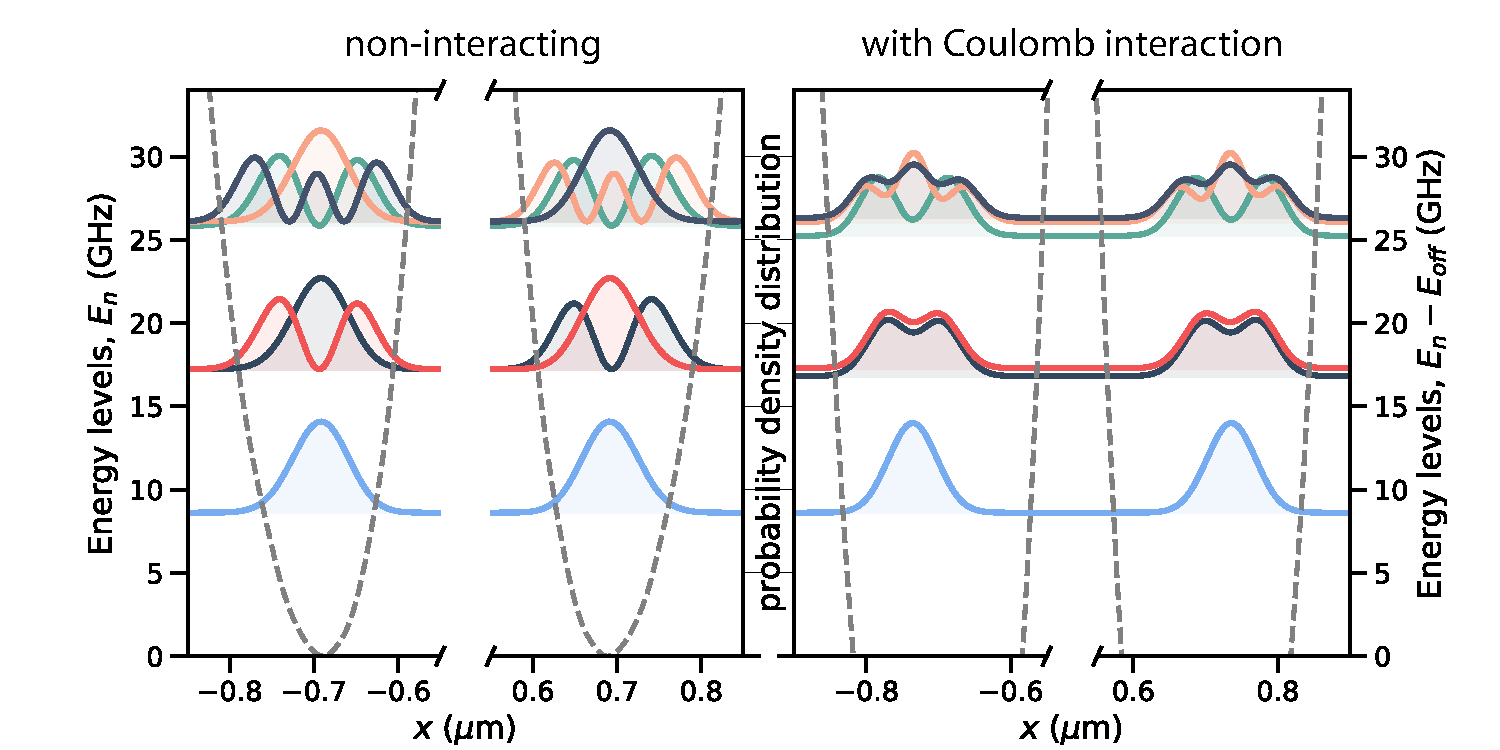
\includegraphics[width=0.49\textwidth]{figure2.pdf}
\caption{\label{fig3} (a) Figure caption.}
\end{figure}

\section{Results and Discussion} % all of us

\begin{figure}
\includegraphics[width=0.49\textwidth]{figure3.pdf}
\caption{\label{fig3} (a) Figure caption.}
\end{figure}

\section{Conclusions} % we can wait to write this one until the end

\section{\label{sec:level1}Problem: Many-level system interacting with EM field}

We start with the following problem in general form: we have a quantum-mechanical system described with Hamiltonian $H_0$ and states $\ket{n}$ being eigenfunctions of $H_0$.
\begin{equation*}
H_0 \ket{n} = E_n \ket{n}
\end{equation*}
We would like to know how these states evolve in time in the presence of a time-varying electric field. The interaction of quantum systems with electric fields is described by the Hamiltonian $ H_i = - \vb{E}(t) \vb{d}$, where $\vb{E}(t) = \vb{\mathcal{E}}_0 \cos \omega t$ and $\vb{d}$ is the dipole moment of the quantum system. Note, here we use dipole approximation (wavelength of the EM field is much larger than characteristic size of the quantum system wavefunction). The evolution of the quantum wavefunction is governed by Schrodinger equation:
\begin{equation}
 i \dot{\psi} = H \psi
\label{eq1}.
\end{equation}
where $H = H_0 + H_i$ (note, $\hbar = 1$). We seek the solution in the form $\psi(t) = \sum_n C_n(t) e^{-i E_n t}$. We evolve this solution through Eq.~\ref{eq1} and get the following answer:
\begin{equation}
 i \dot{C_m} = -\frac{1}{2} \vb{\mathcal{E}}_0 \sum_{\alpha} \sum_{n} C_n e^{i \omega_{mn} t + i \alpha \omega t} \vb{d}_{mn}
\label{eq2},
\end{equation}
\begin{equation}
 \braket{m}{n} = \delta_{mn}, \mel{m}{\vb{d}}{n} = \vb{d}_{mn}, E_m - E_n = \omega_{mn}
\end{equation}
Here we used $\cos \omega t = \frac{1}{2} \sum_{\alpha = \pm} e^{i \alpha \omega t}$. Lets assume the system is in the ground state at $t = 0$, so $C_n(0) = \delta_{n1}$. We integrate Eq.~\ref{eq2} and get an expression:
\begin{equation}
 C_m = \frac{i}{2} \vb{\mathcal{E}}_0 \sum_{\alpha} \vb{d}_{m1} \frac{e^{i (\omega_{mn} + \alpha \omega) t} - 1}{i (\omega_{m1} + \alpha \omega)} 
\label{eq3}.
\end{equation}
An important condition here is:
\begin{equation}
\abs{\frac{\vb{\mathcal{E}}_0 \vb{d}_{m1}}{\omega_{m1} \pm \omega}} \ll 1
\label{eq4},
\end{equation}
which defines the 2-level approximation

\section{Appendix A}
Description of classical two-body calculation


\begin{acknowledgments}
We are grateful to M.I. Dykman and S.A. Lyon for illuminating discussions. The work of MHJ is supported by the U.S. Department of Energy, Office of Science, office of Nuclear Physics under grant No. DE-SC0021152 and U.S. National Science Foundation Grants No. PHY-1404159 and PHY-2013047. JP acknowledges support from the National Science Foundation via grant number DMR-2003815 as well as the valuable support of the Cowen Family Endowment at MSU. The work of NRB is supported by a sponsored research grant from EeroQ Corp. JP and NRB thank J.R. Lane and J.M. Kitzman for illuminating discussions.
\end{acknowledgments}
\bibliography{apssamp}% Produces the bibliography via BibTeX.

\end{document}
%
% ****** End of file apssamp.tex ******
